% Graphic for TeX using PGF
% Title: /home/tomgli/workspace/github.com/bachopp/thesis/files/chapters/background/graphs/reactdiffdiagram.dia
% Creator: Dia v0.97.3
% CreationDate: Sat Apr 23 13:17:49 2016
% For: tomgli
% \usepackage{tikz}
% The following commands are not supported in PSTricks at present
% We define them conditionally, so when they are implemented,
% this pgf file will use them.
\ifx\du\undefined
  \newlength{\du}
\fi
\setlength{\du}{15\unitlength}
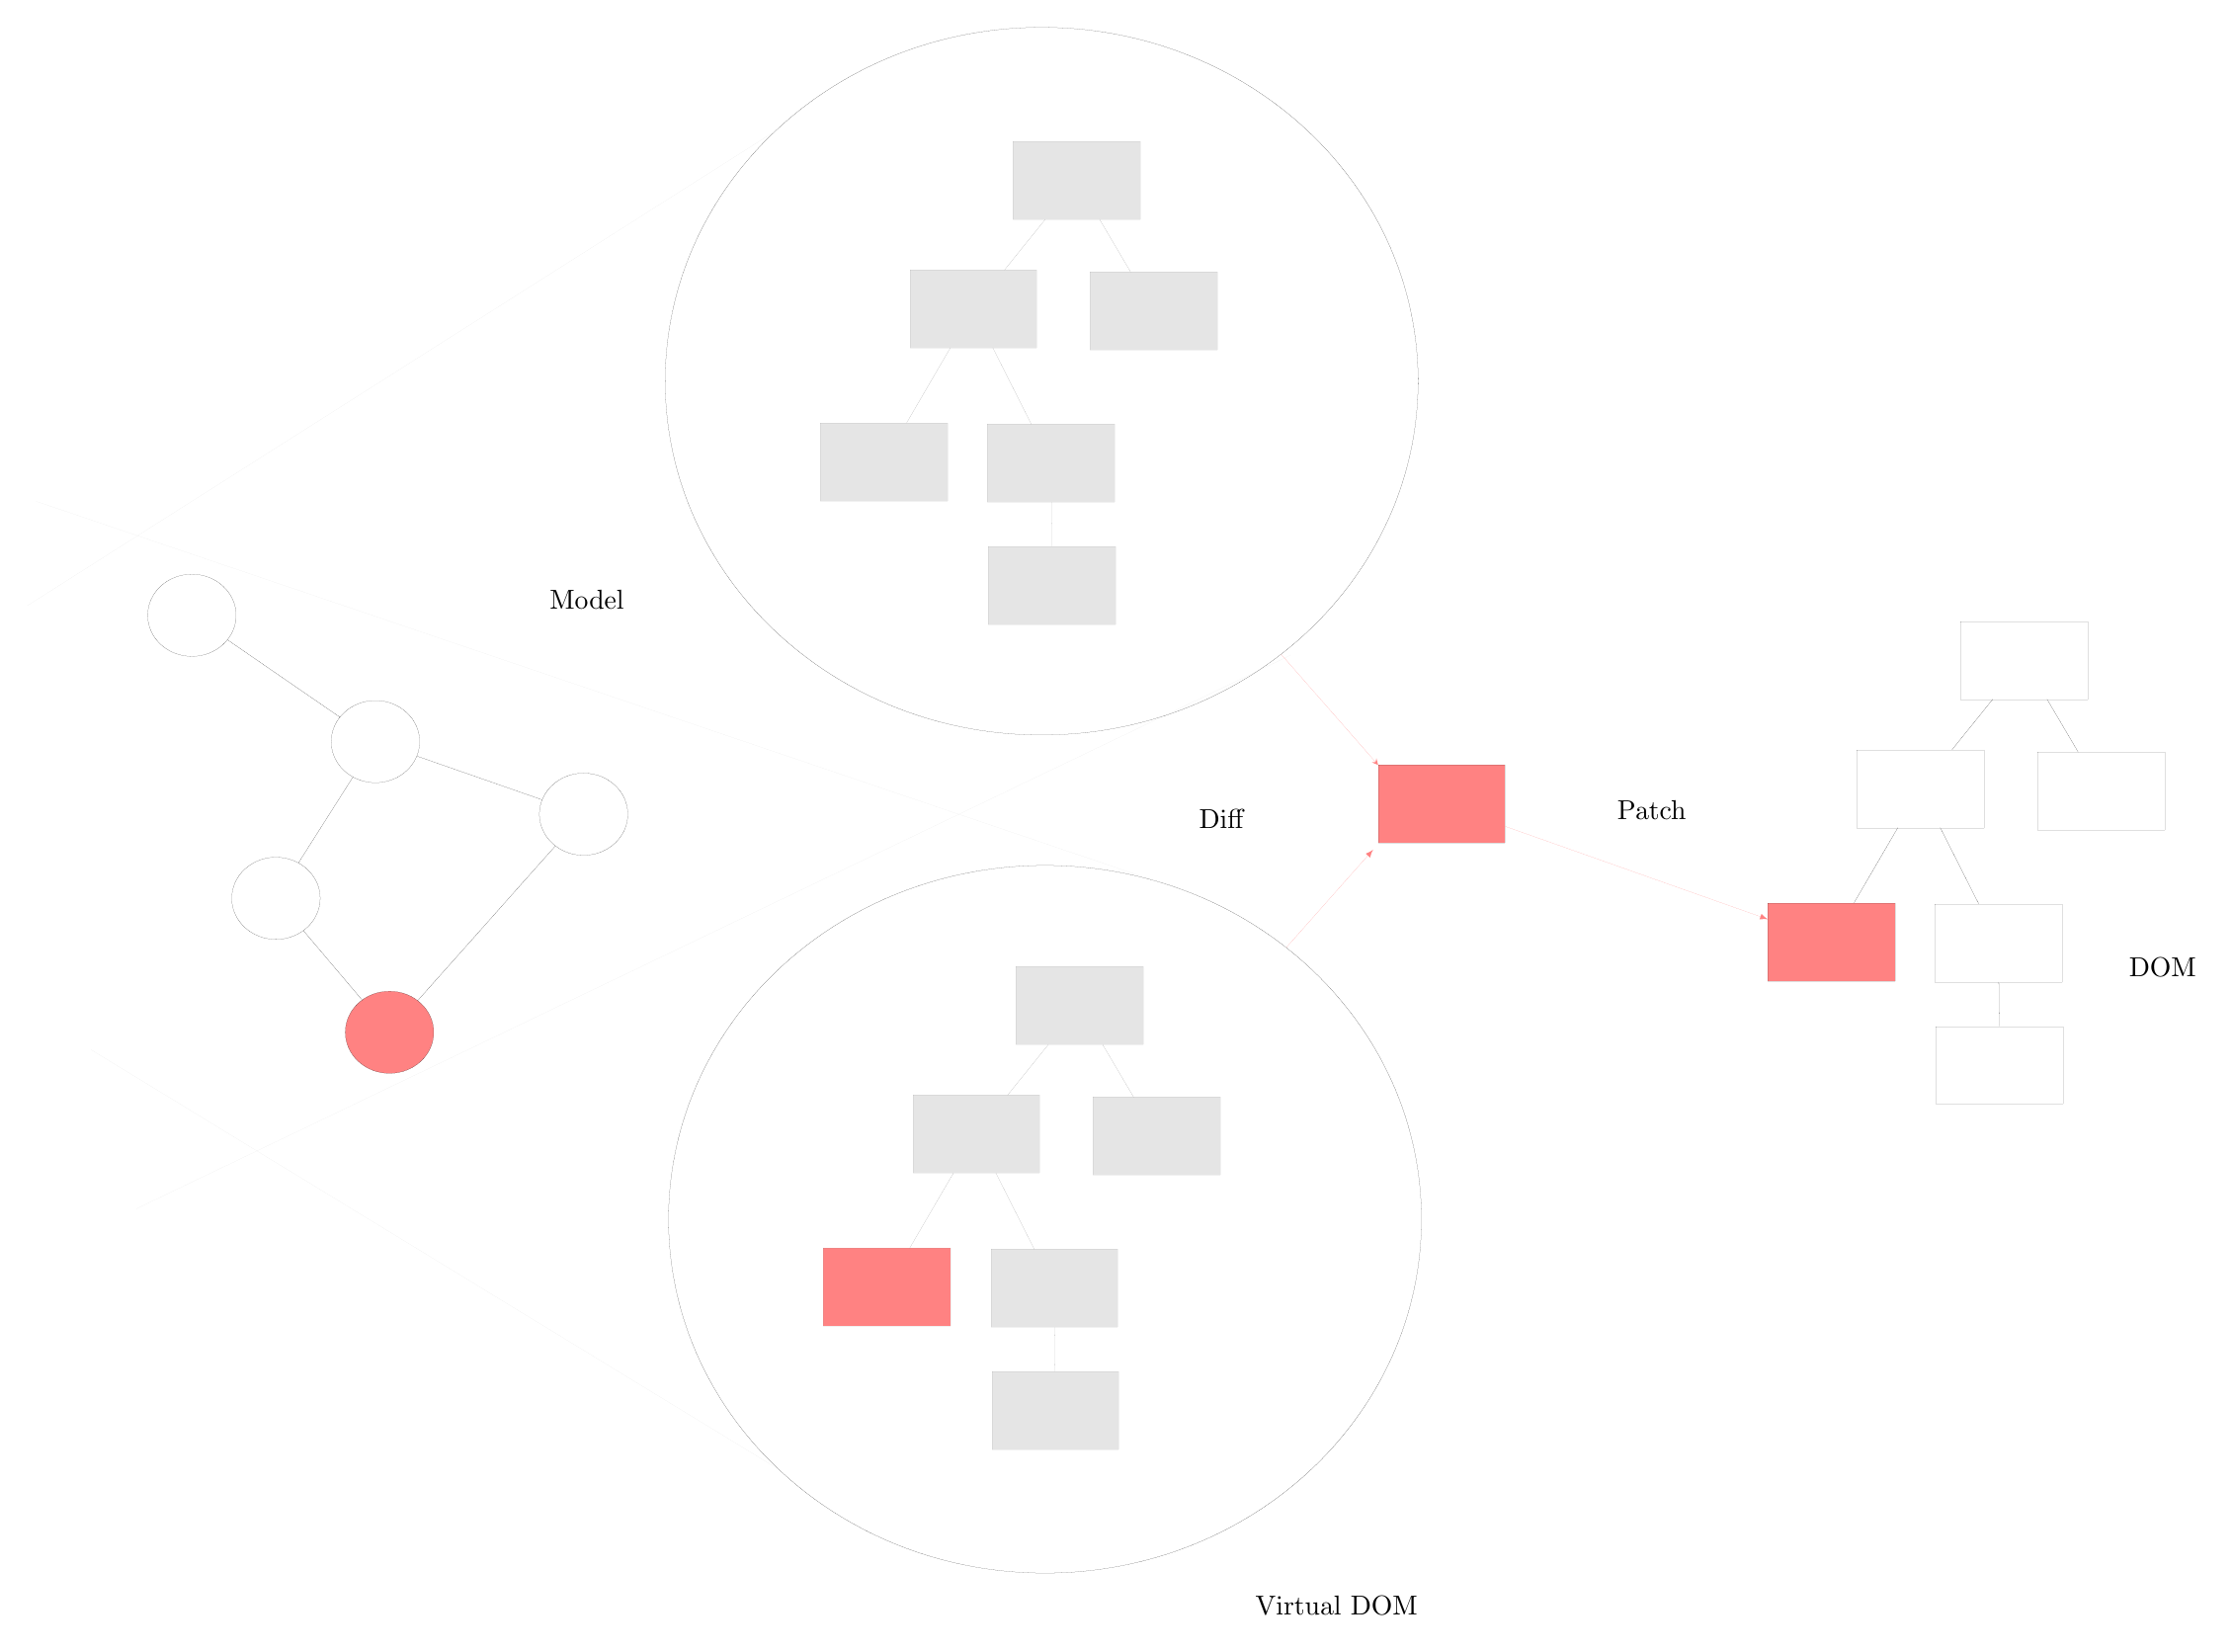
\begin{tikzpicture}
\pgftransformxscale{1.000000}
\pgftransformyscale{-1.000000}
\definecolor{dialinecolor}{rgb}{0.000000, 0.000000, 0.000000}
\pgfsetstrokecolor{dialinecolor}
\definecolor{dialinecolor}{rgb}{1.000000, 1.000000, 1.000000}
\pgfsetfillcolor{dialinecolor}
% setfont left to latex
\definecolor{dialinecolor}{rgb}{0.000000, 0.000000, 0.000000}
\pgfsetstrokecolor{dialinecolor}
\node[anchor=west] at (44.191500\du,20.931300\du){Patch};
% setfont left to latex
\definecolor{dialinecolor}{rgb}{0.000000, 0.000000, 0.000000}
\pgfsetstrokecolor{dialinecolor}
\node[anchor=west] at (33.990300\du,21.142600\du){Diff};
% setfont left to latex
\definecolor{dialinecolor}{rgb}{0.000000, 0.000000, 0.000000}
\pgfsetstrokecolor{dialinecolor}
\node[anchor=west] at (56.666500\du,24.761300\du){DOM};
% setfont left to latex
\definecolor{dialinecolor}{rgb}{0.000000, 0.000000, 0.000000}
\pgfsetstrokecolor{dialinecolor}
\node[anchor=west] at (35.366500\du,40.311300\du){Virtual DOM};
% setfont left to latex
\definecolor{dialinecolor}{rgb}{0.000000, 0.000000, 0.000000}
\pgfsetstrokecolor{dialinecolor}
\node at (19.300700\du,15.793600\du){Model};
\definecolor{dialinecolor}{rgb}{1.000000, 0.509804, 0.509804}
\pgfsetfillcolor{dialinecolor}
\pgfpathellipse{\pgfpoint{14.489164\du}{26.338882\du}}{\pgfpoint{1.078364\du}{0\du}}{\pgfpoint{0\du}{1.001682\du}}
\pgfusepath{fill}
\pgfsetlinewidth{0.000200\du}
\pgfsetdash{}{0pt}
\pgfsetdash{}{0pt}
\pgfsetmiterjoin
\definecolor{dialinecolor}{rgb}{0.000000, 0.000000, 0.000000}
\pgfsetstrokecolor{dialinecolor}
\pgfpathellipse{\pgfpoint{14.489164\du}{26.338882\du}}{\pgfpoint{1.078364\du}{0\du}}{\pgfpoint{0\du}{1.001682\du}}
\pgfusepath{stroke}
% setfont left to latex
\definecolor{dialinecolor}{rgb}{0.000000, 0.000000, 0.000000}
\pgfsetstrokecolor{dialinecolor}
\node at (14.489164\du,26.511104\du){};
\definecolor{dialinecolor}{rgb}{1.000000, 1.000000, 1.000000}
\pgfsetfillcolor{dialinecolor}
\pgfpathellipse{\pgfpoint{11.720864\du}{23.072282\du}}{\pgfpoint{1.078364\du}{0\du}}{\pgfpoint{0\du}{1.001682\du}}
\pgfusepath{fill}
\pgfsetlinewidth{0.000200\du}
\pgfsetdash{}{0pt}
\pgfsetdash{}{0pt}
\pgfsetmiterjoin
\definecolor{dialinecolor}{rgb}{0.000000, 0.000000, 0.000000}
\pgfsetstrokecolor{dialinecolor}
\pgfpathellipse{\pgfpoint{11.720864\du}{23.072282\du}}{\pgfpoint{1.078364\du}{0\du}}{\pgfpoint{0\du}{1.001682\du}}
\pgfusepath{stroke}
% setfont left to latex
\definecolor{dialinecolor}{rgb}{0.000000, 0.000000, 0.000000}
\pgfsetstrokecolor{dialinecolor}
\node at (11.720864\du,23.244504\du){};
\definecolor{dialinecolor}{rgb}{1.000000, 1.000000, 1.000000}
\pgfsetfillcolor{dialinecolor}
\pgfpathellipse{\pgfpoint{14.145864\du}{19.252282\du}}{\pgfpoint{1.078364\du}{0\du}}{\pgfpoint{0\du}{1.001682\du}}
\pgfusepath{fill}
\pgfsetlinewidth{0.000200\du}
\pgfsetdash{}{0pt}
\pgfsetdash{}{0pt}
\pgfsetmiterjoin
\definecolor{dialinecolor}{rgb}{0.000000, 0.000000, 0.000000}
\pgfsetstrokecolor{dialinecolor}
\pgfpathellipse{\pgfpoint{14.145864\du}{19.252282\du}}{\pgfpoint{1.078364\du}{0\du}}{\pgfpoint{0\du}{1.001682\du}}
\pgfusepath{stroke}
% setfont left to latex
\definecolor{dialinecolor}{rgb}{0.000000, 0.000000, 0.000000}
\pgfsetstrokecolor{dialinecolor}
\node at (14.145864\du,19.424504\du){};
\definecolor{dialinecolor}{rgb}{1.000000, 1.000000, 1.000000}
\pgfsetfillcolor{dialinecolor}
\pgfpathellipse{\pgfpoint{19.220864\du}{21.022282\du}}{\pgfpoint{1.078364\du}{0\du}}{\pgfpoint{0\du}{1.001682\du}}
\pgfusepath{fill}
\pgfsetlinewidth{0.000200\du}
\pgfsetdash{}{0pt}
\pgfsetdash{}{0pt}
\pgfsetmiterjoin
\definecolor{dialinecolor}{rgb}{0.000000, 0.000000, 0.000000}
\pgfsetstrokecolor{dialinecolor}
\pgfpathellipse{\pgfpoint{19.220864\du}{21.022282\du}}{\pgfpoint{1.078364\du}{0\du}}{\pgfpoint{0\du}{1.001682\du}}
\pgfusepath{stroke}
% setfont left to latex
\definecolor{dialinecolor}{rgb}{0.000000, 0.000000, 0.000000}
\pgfsetstrokecolor{dialinecolor}
\node at (19.220864\du,21.194504\du){};
\definecolor{dialinecolor}{rgb}{1.000000, 1.000000, 1.000000}
\pgfsetfillcolor{dialinecolor}
\pgfpathellipse{\pgfpoint{9.670904\du}{16.172282\du}}{\pgfpoint{1.078364\du}{0\du}}{\pgfpoint{0\du}{1.001682\du}}
\pgfusepath{fill}
\pgfsetlinewidth{0.000200\du}
\pgfsetdash{}{0pt}
\pgfsetdash{}{0pt}
\pgfsetmiterjoin
\definecolor{dialinecolor}{rgb}{0.000000, 0.000000, 0.000000}
\pgfsetstrokecolor{dialinecolor}
\pgfpathellipse{\pgfpoint{9.670904\du}{16.172282\du}}{\pgfpoint{1.078364\du}{0\du}}{\pgfpoint{0\du}{1.001682\du}}
\pgfusepath{stroke}
% setfont left to latex
\definecolor{dialinecolor}{rgb}{0.000000, 0.000000, 0.000000}
\pgfsetstrokecolor{dialinecolor}
\node at (9.670904\du,16.344504\du){};
\pgfsetlinewidth{0.000200\du}
\pgfsetdash{}{0pt}
\pgfsetdash{}{0pt}
\pgfsetbuttcap
{
\definecolor{dialinecolor}{rgb}{0.000000, 0.000000, 0.000000}
\pgfsetfillcolor{dialinecolor}
% was here!!!
\definecolor{dialinecolor}{rgb}{0.000000, 0.000000, 0.000000}
\pgfsetstrokecolor{dialinecolor}
\draw (10.537545\du,16.768769\du)--(13.279223\du,18.655795\du);
}
\pgfsetlinewidth{0.000200\du}
\pgfsetdash{}{0pt}
\pgfsetdash{}{0pt}
\pgfsetbuttcap
{
\definecolor{dialinecolor}{rgb}{0.000000, 0.000000, 0.000000}
\pgfsetfillcolor{dialinecolor}
% was here!!!
\definecolor{dialinecolor}{rgb}{0.000000, 0.000000, 0.000000}
\pgfsetstrokecolor{dialinecolor}
\draw (15.155041\du,19.604251\du)--(18.211687\du,20.670313\du);
}
\pgfsetlinewidth{0.000200\du}
\pgfsetdash{}{0pt}
\pgfsetdash{}{0pt}
\pgfsetbuttcap
{
\definecolor{dialinecolor}{rgb}{0.000000, 0.000000, 0.000000}
\pgfsetfillcolor{dialinecolor}
% was here!!!
\definecolor{dialinecolor}{rgb}{0.000000, 0.000000, 0.000000}
\pgfsetstrokecolor{dialinecolor}
\draw (13.598226\du,20.114953\du)--(12.268502\du,22.209611\du);
}
\pgfsetlinewidth{0.000200\du}
\pgfsetdash{}{0pt}
\pgfsetdash{}{0pt}
\pgfsetbuttcap
{
\definecolor{dialinecolor}{rgb}{0.000000, 0.000000, 0.000000}
\pgfsetfillcolor{dialinecolor}
% was here!!!
\definecolor{dialinecolor}{rgb}{0.000000, 0.000000, 0.000000}
\pgfsetstrokecolor{dialinecolor}
\draw (12.388101\du,23.859623\du)--(13.821927\du,25.551540\du);
}
\pgfsetlinewidth{0.000200\du}
\pgfsetdash{}{0pt}
\pgfsetdash{}{0pt}
\pgfsetbuttcap
{
\definecolor{dialinecolor}{rgb}{0.000000, 0.000000, 0.000000}
\pgfsetfillcolor{dialinecolor}
% was here!!!
\definecolor{dialinecolor}{rgb}{0.000000, 0.000000, 0.000000}
\pgfsetstrokecolor{dialinecolor}
\draw (15.175930\du,25.567222\du)--(18.534097\du,21.793942\du);
}
\definecolor{dialinecolor}{rgb}{0.898039, 0.898039, 0.898039}
\pgfsetfillcolor{dialinecolor}
\fill (29.767500\du,24.740600\du)--(29.767500\du,26.640600\du)--(32.867500\du,26.640600\du)--(32.867500\du,24.740600\du)--cycle;
\pgfsetlinewidth{0.000200\du}
\pgfsetdash{}{0pt}
\pgfsetdash{}{0pt}
\pgfsetmiterjoin
\definecolor{dialinecolor}{rgb}{0.549020, 0.549020, 0.549020}
\pgfsetstrokecolor{dialinecolor}
\draw (29.767500\du,24.740600\du)--(29.767500\du,26.640600\du)--(32.867500\du,26.640600\du)--(32.867500\du,24.740600\du)--cycle;
% setfont left to latex
\definecolor{dialinecolor}{rgb}{0.000000, 0.000000, 0.000000}
\pgfsetstrokecolor{dialinecolor}
\node at (31.317500\du,25.862822\du){};
\definecolor{dialinecolor}{rgb}{0.898039, 0.898039, 0.898039}
\pgfsetfillcolor{dialinecolor}
\fill (27.242500\du,27.870600\du)--(27.242500\du,29.770600\du)--(30.342500\du,29.770600\du)--(30.342500\du,27.870600\du)--cycle;
\pgfsetlinewidth{0.000200\du}
\pgfsetdash{}{0pt}
\pgfsetdash{}{0pt}
\pgfsetmiterjoin
\definecolor{dialinecolor}{rgb}{0.549020, 0.549020, 0.549020}
\pgfsetstrokecolor{dialinecolor}
\draw (27.242500\du,27.870600\du)--(27.242500\du,29.770600\du)--(30.342500\du,29.770600\du)--(30.342500\du,27.870600\du)--cycle;
% setfont left to latex
\definecolor{dialinecolor}{rgb}{0.000000, 0.000000, 0.000000}
\pgfsetstrokecolor{dialinecolor}
\node at (28.792500\du,28.992822\du){};
\definecolor{dialinecolor}{rgb}{0.898039, 0.898039, 0.898039}
\pgfsetfillcolor{dialinecolor}
\fill (31.642500\du,27.920600\du)--(31.642500\du,29.820600\du)--(34.742500\du,29.820600\du)--(34.742500\du,27.920600\du)--cycle;
\pgfsetlinewidth{0.000200\du}
\pgfsetdash{}{0pt}
\pgfsetdash{}{0pt}
\pgfsetmiterjoin
\definecolor{dialinecolor}{rgb}{0.549020, 0.549020, 0.549020}
\pgfsetstrokecolor{dialinecolor}
\draw (31.642500\du,27.920600\du)--(31.642500\du,29.820600\du)--(34.742500\du,29.820600\du)--(34.742500\du,27.920600\du)--cycle;
% setfont left to latex
\definecolor{dialinecolor}{rgb}{0.000000, 0.000000, 0.000000}
\pgfsetstrokecolor{dialinecolor}
\node at (33.192500\du,29.042822\du){};
\definecolor{dialinecolor}{rgb}{1.000000, 0.509804, 0.509804}
\pgfsetfillcolor{dialinecolor}
\fill (25.067500\du,31.600600\du)--(25.067500\du,33.500600\du)--(28.167500\du,33.500600\du)--(28.167500\du,31.600600\du)--cycle;
\pgfsetlinewidth{0.000200\du}
\pgfsetdash{}{0pt}
\pgfsetdash{}{0pt}
\pgfsetmiterjoin
\definecolor{dialinecolor}{rgb}{0.549020, 0.549020, 0.549020}
\pgfsetstrokecolor{dialinecolor}
\draw (25.067500\du,31.600600\du)--(25.067500\du,33.500600\du)--(28.167500\du,33.500600\du)--(28.167500\du,31.600600\du)--cycle;
% setfont left to latex
\definecolor{dialinecolor}{rgb}{0.000000, 0.000000, 0.000000}
\pgfsetstrokecolor{dialinecolor}
\node at (26.617500\du,32.722822\du){};
\definecolor{dialinecolor}{rgb}{0.898039, 0.898039, 0.898039}
\pgfsetfillcolor{dialinecolor}
\fill (29.142500\du,31.630600\du)--(29.142500\du,33.530600\du)--(32.242500\du,33.530600\du)--(32.242500\du,31.630600\du)--cycle;
\pgfsetlinewidth{0.000200\du}
\pgfsetdash{}{0pt}
\pgfsetdash{}{0pt}
\pgfsetmiterjoin
\definecolor{dialinecolor}{rgb}{0.549020, 0.549020, 0.549020}
\pgfsetstrokecolor{dialinecolor}
\draw (29.142500\du,31.630600\du)--(29.142500\du,33.530600\du)--(32.242500\du,33.530600\du)--(32.242500\du,31.630600\du)--cycle;
% setfont left to latex
\definecolor{dialinecolor}{rgb}{0.000000, 0.000000, 0.000000}
\pgfsetstrokecolor{dialinecolor}
\node at (30.692500\du,32.752822\du){};
\definecolor{dialinecolor}{rgb}{0.898039, 0.898039, 0.898039}
\pgfsetfillcolor{dialinecolor}
\fill (29.167500\du,34.610600\du)--(29.167500\du,36.510600\du)--(32.267500\du,36.510600\du)--(32.267500\du,34.610600\du)--cycle;
\pgfsetlinewidth{0.000200\du}
\pgfsetdash{}{0pt}
\pgfsetdash{}{0pt}
\pgfsetmiterjoin
\definecolor{dialinecolor}{rgb}{0.549020, 0.549020, 0.549020}
\pgfsetstrokecolor{dialinecolor}
\draw (29.167500\du,34.610600\du)--(29.167500\du,36.510600\du)--(32.267500\du,36.510600\du)--(32.267500\du,34.610600\du)--cycle;
% setfont left to latex
\definecolor{dialinecolor}{rgb}{0.000000, 0.000000, 0.000000}
\pgfsetstrokecolor{dialinecolor}
\node at (30.717500\du,35.732822\du){};
\pgfsetlinewidth{0.000200\du}
\pgfsetdash{}{0pt}
\pgfsetdash{}{0pt}
\pgfsetbuttcap
{
\definecolor{dialinecolor}{rgb}{0.549020, 0.549020, 0.549020}
\pgfsetfillcolor{dialinecolor}
% was here!!!
\definecolor{dialinecolor}{rgb}{0.549020, 0.549020, 0.549020}
\pgfsetstrokecolor{dialinecolor}
\draw (30.700465\du,33.530038\du)--(30.709535\du,34.611162\du);
}
\pgfsetlinewidth{0.000200\du}
\pgfsetdash{}{0pt}
\pgfsetdash{}{0pt}
\pgfsetbuttcap
{
\definecolor{dialinecolor}{rgb}{0.549020, 0.549020, 0.549020}
\pgfsetfillcolor{dialinecolor}
% was here!!!
\definecolor{dialinecolor}{rgb}{0.549020, 0.549020, 0.549020}
\pgfsetstrokecolor{dialinecolor}
\draw (28.239192\du,29.769492\du)--(27.170808\du,31.601708\du);
}
\pgfsetlinewidth{0.000200\du}
\pgfsetdash{}{0pt}
\pgfsetdash{}{0pt}
\pgfsetbuttcap
{
\definecolor{dialinecolor}{rgb}{0.549020, 0.549020, 0.549020}
\pgfsetfillcolor{dialinecolor}
% was here!!!
\definecolor{dialinecolor}{rgb}{0.549020, 0.549020, 0.549020}
\pgfsetstrokecolor{dialinecolor}
\draw (29.272139\du,29.769780\du)--(30.212861\du,31.631420\du);
}
\pgfsetlinewidth{0.000200\du}
\pgfsetdash{}{0pt}
\pgfsetdash{}{0pt}
\pgfsetbuttcap
{
\definecolor{dialinecolor}{rgb}{0.549020, 0.549020, 0.549020}
\pgfsetfillcolor{dialinecolor}
% was here!!!
\definecolor{dialinecolor}{rgb}{0.549020, 0.549020, 0.549020}
\pgfsetstrokecolor{dialinecolor}
\draw (30.551863\du,26.639687\du)--(29.558137\du,27.871513\du);
}
\pgfsetlinewidth{0.000200\du}
\pgfsetdash{}{0pt}
\pgfsetdash{}{0pt}
\pgfsetbuttcap
{
\definecolor{dialinecolor}{rgb}{0.549020, 0.549020, 0.549020}
\pgfsetfillcolor{dialinecolor}
% was here!!!
\definecolor{dialinecolor}{rgb}{0.549020, 0.549020, 0.549020}
\pgfsetstrokecolor{dialinecolor}
\draw (31.875972\du,26.637768\du)--(32.634028\du,27.923432\du);
}
\definecolor{dialinecolor}{rgb}{0.898039, 0.898039, 0.898039}
\pgfsetfillcolor{dialinecolor}
\fill (29.692500\du,4.620560\du)--(29.692500\du,6.520560\du)--(32.792500\du,6.520560\du)--(32.792500\du,4.620560\du)--cycle;
\pgfsetlinewidth{0.000200\du}
\pgfsetdash{}{0pt}
\pgfsetdash{}{0pt}
\pgfsetmiterjoin
\definecolor{dialinecolor}{rgb}{0.549020, 0.549020, 0.549020}
\pgfsetstrokecolor{dialinecolor}
\draw (29.692500\du,4.620560\du)--(29.692500\du,6.520560\du)--(32.792500\du,6.520560\du)--(32.792500\du,4.620560\du)--cycle;
% setfont left to latex
\definecolor{dialinecolor}{rgb}{0.000000, 0.000000, 0.000000}
\pgfsetstrokecolor{dialinecolor}
\node at (31.242500\du,5.742782\du){};
\definecolor{dialinecolor}{rgb}{0.898039, 0.898039, 0.898039}
\pgfsetfillcolor{dialinecolor}
\fill (27.167500\du,7.750560\du)--(27.167500\du,9.650560\du)--(30.267500\du,9.650560\du)--(30.267500\du,7.750560\du)--cycle;
\pgfsetlinewidth{0.000200\du}
\pgfsetdash{}{0pt}
\pgfsetdash{}{0pt}
\pgfsetmiterjoin
\definecolor{dialinecolor}{rgb}{0.549020, 0.549020, 0.549020}
\pgfsetstrokecolor{dialinecolor}
\draw (27.167500\du,7.750560\du)--(27.167500\du,9.650560\du)--(30.267500\du,9.650560\du)--(30.267500\du,7.750560\du)--cycle;
% setfont left to latex
\definecolor{dialinecolor}{rgb}{0.000000, 0.000000, 0.000000}
\pgfsetstrokecolor{dialinecolor}
\node at (28.717500\du,8.872782\du){};
\definecolor{dialinecolor}{rgb}{0.898039, 0.898039, 0.898039}
\pgfsetfillcolor{dialinecolor}
\fill (31.567500\du,7.800560\du)--(31.567500\du,9.700560\du)--(34.667500\du,9.700560\du)--(34.667500\du,7.800560\du)--cycle;
\pgfsetlinewidth{0.000200\du}
\pgfsetdash{}{0pt}
\pgfsetdash{}{0pt}
\pgfsetmiterjoin
\definecolor{dialinecolor}{rgb}{0.549020, 0.549020, 0.549020}
\pgfsetstrokecolor{dialinecolor}
\draw (31.567500\du,7.800560\du)--(31.567500\du,9.700560\du)--(34.667500\du,9.700560\du)--(34.667500\du,7.800560\du)--cycle;
% setfont left to latex
\definecolor{dialinecolor}{rgb}{0.000000, 0.000000, 0.000000}
\pgfsetstrokecolor{dialinecolor}
\node at (33.117500\du,8.922782\du){};
\definecolor{dialinecolor}{rgb}{0.898039, 0.898039, 0.898039}
\pgfsetfillcolor{dialinecolor}
\fill (24.992500\du,11.480600\du)--(24.992500\du,13.380600\du)--(28.092500\du,13.380600\du)--(28.092500\du,11.480600\du)--cycle;
\pgfsetlinewidth{0.000200\du}
\pgfsetdash{}{0pt}
\pgfsetdash{}{0pt}
\pgfsetmiterjoin
\definecolor{dialinecolor}{rgb}{0.549020, 0.549020, 0.549020}
\pgfsetstrokecolor{dialinecolor}
\draw (24.992500\du,11.480600\du)--(24.992500\du,13.380600\du)--(28.092500\du,13.380600\du)--(28.092500\du,11.480600\du)--cycle;
% setfont left to latex
\definecolor{dialinecolor}{rgb}{0.000000, 0.000000, 0.000000}
\pgfsetstrokecolor{dialinecolor}
\node at (26.542500\du,12.602822\du){};
\definecolor{dialinecolor}{rgb}{0.898039, 0.898039, 0.898039}
\pgfsetfillcolor{dialinecolor}
\fill (29.067500\du,11.510600\du)--(29.067500\du,13.410600\du)--(32.167500\du,13.410600\du)--(32.167500\du,11.510600\du)--cycle;
\pgfsetlinewidth{0.000200\du}
\pgfsetdash{}{0pt}
\pgfsetdash{}{0pt}
\pgfsetmiterjoin
\definecolor{dialinecolor}{rgb}{0.549020, 0.549020, 0.549020}
\pgfsetstrokecolor{dialinecolor}
\draw (29.067500\du,11.510600\du)--(29.067500\du,13.410600\du)--(32.167500\du,13.410600\du)--(32.167500\du,11.510600\du)--cycle;
% setfont left to latex
\definecolor{dialinecolor}{rgb}{0.000000, 0.000000, 0.000000}
\pgfsetstrokecolor{dialinecolor}
\node at (30.617500\du,12.632822\du){};
\definecolor{dialinecolor}{rgb}{0.898039, 0.898039, 0.898039}
\pgfsetfillcolor{dialinecolor}
\fill (29.092500\du,14.490600\du)--(29.092500\du,16.390600\du)--(32.192500\du,16.390600\du)--(32.192500\du,14.490600\du)--cycle;
\pgfsetlinewidth{0.000200\du}
\pgfsetdash{}{0pt}
\pgfsetdash{}{0pt}
\pgfsetmiterjoin
\definecolor{dialinecolor}{rgb}{0.549020, 0.549020, 0.549020}
\pgfsetstrokecolor{dialinecolor}
\draw (29.092500\du,14.490600\du)--(29.092500\du,16.390600\du)--(32.192500\du,16.390600\du)--(32.192500\du,14.490600\du)--cycle;
% setfont left to latex
\definecolor{dialinecolor}{rgb}{0.000000, 0.000000, 0.000000}
\pgfsetstrokecolor{dialinecolor}
\node at (30.642500\du,15.612822\du){};
\pgfsetlinewidth{0.000200\du}
\pgfsetdash{}{0pt}
\pgfsetdash{}{0pt}
\pgfsetbuttcap
{
\definecolor{dialinecolor}{rgb}{0.549020, 0.549020, 0.549020}
\pgfsetfillcolor{dialinecolor}
% was here!!!
\definecolor{dialinecolor}{rgb}{0.549020, 0.549020, 0.549020}
\pgfsetstrokecolor{dialinecolor}
\draw (30.625465\du,13.410038\du)--(30.634535\du,14.491162\du);
}
\pgfsetlinewidth{0.000200\du}
\pgfsetdash{}{0pt}
\pgfsetdash{}{0pt}
\pgfsetbuttcap
{
\definecolor{dialinecolor}{rgb}{0.549020, 0.549020, 0.549020}
\pgfsetfillcolor{dialinecolor}
% was here!!!
\definecolor{dialinecolor}{rgb}{0.549020, 0.549020, 0.549020}
\pgfsetstrokecolor{dialinecolor}
\draw (28.164192\du,9.649462\du)--(27.095808\du,11.481698\du);
}
\pgfsetlinewidth{0.000200\du}
\pgfsetdash{}{0pt}
\pgfsetdash{}{0pt}
\pgfsetbuttcap
{
\definecolor{dialinecolor}{rgb}{0.549020, 0.549020, 0.549020}
\pgfsetfillcolor{dialinecolor}
% was here!!!
\definecolor{dialinecolor}{rgb}{0.549020, 0.549020, 0.549020}
\pgfsetstrokecolor{dialinecolor}
\draw (29.197139\du,9.649750\du)--(30.137861\du,11.511410\du);
}
\pgfsetlinewidth{0.000200\du}
\pgfsetdash{}{0pt}
\pgfsetdash{}{0pt}
\pgfsetbuttcap
{
\definecolor{dialinecolor}{rgb}{0.549020, 0.549020, 0.549020}
\pgfsetfillcolor{dialinecolor}
% was here!!!
\definecolor{dialinecolor}{rgb}{0.549020, 0.549020, 0.549020}
\pgfsetstrokecolor{dialinecolor}
\draw (30.476863\du,6.519647\du)--(29.483137\du,7.751473\du);
}
\pgfsetlinewidth{0.000200\du}
\pgfsetdash{}{0pt}
\pgfsetdash{}{0pt}
\pgfsetbuttcap
{
\definecolor{dialinecolor}{rgb}{0.549020, 0.549020, 0.549020}
\pgfsetfillcolor{dialinecolor}
% was here!!!
\definecolor{dialinecolor}{rgb}{0.549020, 0.549020, 0.549020}
\pgfsetstrokecolor{dialinecolor}
\draw (31.800972\du,6.517728\du)--(32.559028\du,7.803392\du);
}
\definecolor{dialinecolor}{rgb}{1.000000, 0.509804, 0.509804}
\pgfsetfillcolor{dialinecolor}
\fill (38.592500\du,19.820600\du)--(38.592500\du,21.720600\du)--(41.692500\du,21.720600\du)--(41.692500\du,19.820600\du)--cycle;
\pgfsetlinewidth{0.000200\du}
\pgfsetdash{}{0pt}
\pgfsetdash{}{0pt}
\pgfsetmiterjoin
\definecolor{dialinecolor}{rgb}{0.000000, 0.000000, 0.000000}
\pgfsetstrokecolor{dialinecolor}
\draw (38.592500\du,19.820600\du)--(38.592500\du,21.720600\du)--(41.692500\du,21.720600\du)--(41.692500\du,19.820600\du)--cycle;
% setfont left to latex
\definecolor{dialinecolor}{rgb}{0.000000, 0.000000, 0.000000}
\pgfsetstrokecolor{dialinecolor}
\node at (40.142500\du,20.942822\du){};
\definecolor{dialinecolor}{rgb}{1.000000, 1.000000, 1.000000}
\pgfsetfillcolor{dialinecolor}
\fill (52.792500\du,16.320600\du)--(52.792500\du,18.220600\du)--(55.892500\du,18.220600\du)--(55.892500\du,16.320600\du)--cycle;
\pgfsetlinewidth{0.000200\du}
\pgfsetdash{}{0pt}
\pgfsetdash{}{0pt}
\pgfsetmiterjoin
\definecolor{dialinecolor}{rgb}{0.000000, 0.000000, 0.000000}
\pgfsetstrokecolor{dialinecolor}
\draw (52.792500\du,16.320600\du)--(52.792500\du,18.220600\du)--(55.892500\du,18.220600\du)--(55.892500\du,16.320600\du)--cycle;
% setfont left to latex
\definecolor{dialinecolor}{rgb}{0.000000, 0.000000, 0.000000}
\pgfsetstrokecolor{dialinecolor}
\node at (54.342500\du,17.442822\du){};
\definecolor{dialinecolor}{rgb}{1.000000, 1.000000, 1.000000}
\pgfsetfillcolor{dialinecolor}
\fill (50.267500\du,19.450600\du)--(50.267500\du,21.350600\du)--(53.367500\du,21.350600\du)--(53.367500\du,19.450600\du)--cycle;
\pgfsetlinewidth{0.000200\du}
\pgfsetdash{}{0pt}
\pgfsetdash{}{0pt}
\pgfsetmiterjoin
\definecolor{dialinecolor}{rgb}{0.000000, 0.000000, 0.000000}
\pgfsetstrokecolor{dialinecolor}
\draw (50.267500\du,19.450600\du)--(50.267500\du,21.350600\du)--(53.367500\du,21.350600\du)--(53.367500\du,19.450600\du)--cycle;
% setfont left to latex
\definecolor{dialinecolor}{rgb}{0.000000, 0.000000, 0.000000}
\pgfsetstrokecolor{dialinecolor}
\node at (51.817500\du,20.572822\du){};
\definecolor{dialinecolor}{rgb}{1.000000, 1.000000, 1.000000}
\pgfsetfillcolor{dialinecolor}
\fill (54.667500\du,19.500600\du)--(54.667500\du,21.400600\du)--(57.767500\du,21.400600\du)--(57.767500\du,19.500600\du)--cycle;
\pgfsetlinewidth{0.000200\du}
\pgfsetdash{}{0pt}
\pgfsetdash{}{0pt}
\pgfsetmiterjoin
\definecolor{dialinecolor}{rgb}{0.000000, 0.000000, 0.000000}
\pgfsetstrokecolor{dialinecolor}
\draw (54.667500\du,19.500600\du)--(54.667500\du,21.400600\du)--(57.767500\du,21.400600\du)--(57.767500\du,19.500600\du)--cycle;
% setfont left to latex
\definecolor{dialinecolor}{rgb}{0.000000, 0.000000, 0.000000}
\pgfsetstrokecolor{dialinecolor}
\node at (56.217500\du,20.622822\du){};
\definecolor{dialinecolor}{rgb}{1.000000, 0.509804, 0.509804}
\pgfsetfillcolor{dialinecolor}
\fill (48.092500\du,23.180600\du)--(48.092500\du,25.080600\du)--(51.192500\du,25.080600\du)--(51.192500\du,23.180600\du)--cycle;
\pgfsetlinewidth{0.000200\du}
\pgfsetdash{}{0pt}
\pgfsetdash{}{0pt}
\pgfsetmiterjoin
\definecolor{dialinecolor}{rgb}{0.000000, 0.000000, 0.000000}
\pgfsetstrokecolor{dialinecolor}
\draw (48.092500\du,23.180600\du)--(48.092500\du,25.080600\du)--(51.192500\du,25.080600\du)--(51.192500\du,23.180600\du)--cycle;
% setfont left to latex
\definecolor{dialinecolor}{rgb}{0.000000, 0.000000, 0.000000}
\pgfsetstrokecolor{dialinecolor}
\node at (49.642500\du,24.302822\du){};
\definecolor{dialinecolor}{rgb}{1.000000, 1.000000, 1.000000}
\pgfsetfillcolor{dialinecolor}
\fill (52.167500\du,23.210600\du)--(52.167500\du,25.110600\du)--(55.267500\du,25.110600\du)--(55.267500\du,23.210600\du)--cycle;
\pgfsetlinewidth{0.000200\du}
\pgfsetdash{}{0pt}
\pgfsetdash{}{0pt}
\pgfsetmiterjoin
\definecolor{dialinecolor}{rgb}{0.000000, 0.000000, 0.000000}
\pgfsetstrokecolor{dialinecolor}
\draw (52.167500\du,23.210600\du)--(52.167500\du,25.110600\du)--(55.267500\du,25.110600\du)--(55.267500\du,23.210600\du)--cycle;
% setfont left to latex
\definecolor{dialinecolor}{rgb}{0.000000, 0.000000, 0.000000}
\pgfsetstrokecolor{dialinecolor}
\node at (53.717500\du,24.332822\du){};
\definecolor{dialinecolor}{rgb}{1.000000, 1.000000, 1.000000}
\pgfsetfillcolor{dialinecolor}
\fill (52.192500\du,26.190600\du)--(52.192500\du,28.090600\du)--(55.292500\du,28.090600\du)--(55.292500\du,26.190600\du)--cycle;
\pgfsetlinewidth{0.000200\du}
\pgfsetdash{}{0pt}
\pgfsetdash{}{0pt}
\pgfsetmiterjoin
\definecolor{dialinecolor}{rgb}{0.000000, 0.000000, 0.000000}
\pgfsetstrokecolor{dialinecolor}
\draw (52.192500\du,26.190600\du)--(52.192500\du,28.090600\du)--(55.292500\du,28.090600\du)--(55.292500\du,26.190600\du)--cycle;
% setfont left to latex
\definecolor{dialinecolor}{rgb}{0.000000, 0.000000, 0.000000}
\pgfsetstrokecolor{dialinecolor}
\node at (53.742500\du,27.312822\du){};
\pgfsetlinewidth{0.000200\du}
\pgfsetdash{}{0pt}
\pgfsetdash{}{0pt}
\pgfsetbuttcap
{
\definecolor{dialinecolor}{rgb}{0.000000, 0.000000, 0.000000}
\pgfsetfillcolor{dialinecolor}
% was here!!!
\definecolor{dialinecolor}{rgb}{0.000000, 0.000000, 0.000000}
\pgfsetstrokecolor{dialinecolor}
\draw (53.725465\du,25.110038\du)--(53.734535\du,26.191162\du);
}
\pgfsetlinewidth{0.000200\du}
\pgfsetdash{}{0pt}
\pgfsetdash{}{0pt}
\pgfsetbuttcap
{
\definecolor{dialinecolor}{rgb}{0.000000, 0.000000, 0.000000}
\pgfsetfillcolor{dialinecolor}
% was here!!!
\definecolor{dialinecolor}{rgb}{0.000000, 0.000000, 0.000000}
\pgfsetstrokecolor{dialinecolor}
\draw (51.264192\du,21.349492\du)--(50.195808\du,23.181708\du);
}
\pgfsetlinewidth{0.000200\du}
\pgfsetdash{}{0pt}
\pgfsetdash{}{0pt}
\pgfsetbuttcap
{
\definecolor{dialinecolor}{rgb}{0.000000, 0.000000, 0.000000}
\pgfsetfillcolor{dialinecolor}
% was here!!!
\definecolor{dialinecolor}{rgb}{0.000000, 0.000000, 0.000000}
\pgfsetstrokecolor{dialinecolor}
\draw (52.297139\du,21.349780\du)--(53.237861\du,23.211420\du);
}
\pgfsetlinewidth{0.000200\du}
\pgfsetdash{}{0pt}
\pgfsetdash{}{0pt}
\pgfsetbuttcap
{
\definecolor{dialinecolor}{rgb}{0.000000, 0.000000, 0.000000}
\pgfsetfillcolor{dialinecolor}
% was here!!!
\definecolor{dialinecolor}{rgb}{0.000000, 0.000000, 0.000000}
\pgfsetstrokecolor{dialinecolor}
\draw (53.576863\du,18.219687\du)--(52.583137\du,19.451513\du);
}
\pgfsetlinewidth{0.000200\du}
\pgfsetdash{}{0pt}
\pgfsetdash{}{0pt}
\pgfsetbuttcap
{
\definecolor{dialinecolor}{rgb}{0.000000, 0.000000, 0.000000}
\pgfsetfillcolor{dialinecolor}
% was here!!!
\definecolor{dialinecolor}{rgb}{0.000000, 0.000000, 0.000000}
\pgfsetstrokecolor{dialinecolor}
\draw (54.900972\du,18.217768\du)--(55.659028\du,19.503432\du);
}
\pgfsetlinewidth{0.000200\du}
\pgfsetdash{}{0pt}
\pgfsetdash{}{0pt}
\pgfsetbuttcap
{
\definecolor{dialinecolor}{rgb}{0.898039, 0.898039, 0.898039}
\pgfsetfillcolor{dialinecolor}
% was here!!!
\definecolor{dialinecolor}{rgb}{0.898039, 0.898039, 0.898039}
\pgfsetstrokecolor{dialinecolor}
\draw (8.317540\du,30.640600\du)--(36.467500\du,17.140600\du);
}
\pgfsetlinewidth{0.000200\du}
\pgfsetdash{}{0pt}
\pgfsetdash{}{0pt}
\pgfsetmiterjoin
\definecolor{dialinecolor}{rgb}{0.000000, 0.000000, 0.000000}
\pgfsetstrokecolor{dialinecolor}
\pgfpathellipse{\pgfpoint{30.389164\du}{10.463882\du}}{\pgfpoint{9.178364\du}{0\du}}{\pgfpoint{0\du}{8.626682\du}}
\pgfusepath{stroke}
% setfont left to latex
\definecolor{dialinecolor}{rgb}{0.000000, 0.000000, 0.000000}
\pgfsetstrokecolor{dialinecolor}
\node at (30.389164\du,10.636104\du){};
\pgfsetlinewidth{0.000200\du}
\pgfsetdash{}{0pt}
\pgfsetdash{}{0pt}
\pgfsetmiterjoin
\definecolor{dialinecolor}{rgb}{0.000000, 0.000000, 0.000000}
\pgfsetstrokecolor{dialinecolor}
\pgfpathellipse{\pgfpoint{30.470864\du}{30.897282\du}}{\pgfpoint{9.178364\du}{0\du}}{\pgfpoint{0\du}{8.626682\du}}
\pgfusepath{stroke}
% setfont left to latex
\definecolor{dialinecolor}{rgb}{0.000000, 0.000000, 0.000000}
\pgfsetstrokecolor{dialinecolor}
\node at (30.470864\du,31.069504\du){};
\pgfsetlinewidth{0.000200\du}
\pgfsetdash{}{0pt}
\pgfsetdash{}{0pt}
\pgfsetbuttcap
{
\definecolor{dialinecolor}{rgb}{0.898039, 0.898039, 0.898039}
\pgfsetfillcolor{dialinecolor}
% was here!!!
\definecolor{dialinecolor}{rgb}{0.898039, 0.898039, 0.898039}
\pgfsetstrokecolor{dialinecolor}
\draw (5.867540\du,13.390600\du)--(33.983300\du,22.927200\du);
}
\pgfsetlinewidth{0.000200\du}
\pgfsetdash{}{0pt}
\pgfsetdash{}{0pt}
\pgfsetbuttcap
{
\definecolor{dialinecolor}{rgb}{1.000000, 0.509804, 0.509804}
\pgfsetfillcolor{dialinecolor}
% was here!!!
\pgfsetarrowsend{stealth}
\definecolor{dialinecolor}{rgb}{1.000000, 0.509804, 0.509804}
\pgfsetstrokecolor{dialinecolor}
\draw (36.225729\du,17.121063\du)--(38.592500\du,19.820600\du);
}
\pgfsetlinewidth{0.000200\du}
\pgfsetdash{}{0pt}
\pgfsetdash{}{0pt}
\pgfsetbuttcap
{
\definecolor{dialinecolor}{rgb}{1.000000, 0.509804, 0.509804}
\pgfsetfillcolor{dialinecolor}
% was here!!!
\pgfsetarrowsend{latex}
\definecolor{dialinecolor}{rgb}{1.000000, 0.509804, 0.509804}
\pgfsetstrokecolor{dialinecolor}
\draw (36.351691\du,24.273655\du)--(38.467500\du,21.890600\du);
}
\pgfsetlinewidth{0.000200\du}
\pgfsetdash{}{0pt}
\pgfsetdash{}{0pt}
\pgfsetbuttcap
{
\definecolor{dialinecolor}{rgb}{1.000000, 0.509804, 0.509804}
\pgfsetfillcolor{dialinecolor}
% was here!!!
\pgfsetarrowsend{latex}
\definecolor{dialinecolor}{rgb}{1.000000, 0.509804, 0.509804}
\pgfsetstrokecolor{dialinecolor}
\draw (41.692396\du,21.318774\du)--(48.092604\du,23.582426\du);
}
\pgfsetlinewidth{0.000200\du}
\pgfsetdash{}{0pt}
\pgfsetdash{}{0pt}
\pgfsetbuttcap
{
\definecolor{dialinecolor}{rgb}{0.898039, 0.898039, 0.898039}
\pgfsetfillcolor{dialinecolor}
% was here!!!
\definecolor{dialinecolor}{rgb}{0.898039, 0.898039, 0.898039}
\pgfsetstrokecolor{dialinecolor}
\draw (5.659240\du,15.937300\du)--(23.899100\du,4.363900\du);
}
\pgfsetlinewidth{0.000200\du}
\pgfsetdash{}{0pt}
\pgfsetdash{}{0pt}
\pgfsetbuttcap
{
\definecolor{dialinecolor}{rgb}{0.898039, 0.898039, 0.898039}
\pgfsetfillcolor{dialinecolor}
% was here!!!
\definecolor{dialinecolor}{rgb}{0.898039, 0.898039, 0.898039}
\pgfsetstrokecolor{dialinecolor}
\draw (7.211540\du,26.763000\du)--(23.980800\du,36.997200\du);
}
\end{tikzpicture}
